
\documentclass[aspectratio=169]{beamer}
\usepackage[utf8]{inputenc}
\usepackage[T1]{fontenc}
%%%%%%%
% \usepackage{layout}
% \usepackage{lipsum}
%%%%%%%
\usetheme[% Complete settings. Default value in []
% titleimagecolor=red,       % [gray], darkgray, red, blue, green
% titleimagemargin=2mm,      % Distance [2mm]    Frame around title page image
% navigationsymbols=false,   % true   / [false]  Navigation symbols in the foot
% mathseriffont=false,       % true   / [false]  Serif / non-serif math fonts
% foot=true,                 % [true] / false    Footline or not
% nofootslidenum=false       % true   / [false]  Keep slide num even when foot=false
footlogo=false,             % [true] / false    Put LU logo to the left of footer
english=false,              % [true] / false    English / Swedish logo
% LTHlogo=false,             % true   / [false]  Use LTH logo instead of LU on title and end pages.
% blackenumeratenumber=true, % [true] / false    Black enumerate numbers, o.w. Lund bronze
% blackitemmark=false,       % true   / [false]  Black item marks, o.w. Lund bronze
% defaultfont=false,         % true   / [false]  Falls back to default beamer fonts
% sectionframe=true,
]{ulund}
%%%%%%%%%%%%%%%%%%%%% Layout commands 
%%%% Foot
% \ulundfootleft{\insertshortauthor}
% \ulundfootmid{\insertshorttitle}
% \ulundfootright{\insertframenumber}% {\insertframenumber:\inserttotalframenumber}
%%%% Titleimage
\titleimage{Pictures/ULUNDcolor} % Replaces the LU image. Voids option titleimagecolor
%%%%%%%%%%%%%%%%%%%%%%%%%%%%%%%%%%%
\title[B. Regnell, \today]{\selectfont Samverkansråd KB\\ Digitalisering}
\author[\href{https://github.com/bjornregnell/ws-dig}{github.com/bjornregnell/ws-dig}]{%
  Prof. Björn Regnell\newline
  Vicerektor för digitalisering, LTH}
%%%%%%%%%%%%%%%%%%%%%
\usepackage{verbatim}
%%%%%%%%%%%%% Verbatim code box
\usepackage[skins,listings]{tcolorbox}
\tcbuselibrary{listingsutf8}

\usepackage{pgf-pie}

\newcommand{\TitleSlide}{\begin{frame}[plain]\titlepage\end{frame}}

\newcommand{\EndSlide}{\begin{frame}[plain]\endpage\end{frame}}


\newcommand{\Plain}[1]{{\setbeamercolor{background canvas}{bg=black}\begin{frame}[plain]{#1}\end{frame}}}

\newcommand{\ImgFillH}[1]{{\setbeamercolor{background canvas}{bg=black}\begin{frame}[plain]%
{\centering\includegraphics[height=1.0\textheight]{../img/#1}}%
\end{frame}}}

\newcommand{\ImgFillV}[1]{{\setbeamercolor{background canvas}{bg=black}\begin{frame}[plain]%
  {\centering\includegraphics[width=1\textwidth]{../img/#1}}%
  \end{frame}}}
  
% {
% \setbeamercolor{background canvas}{bg=black}
% \begin{frame}[plain]
%   \centering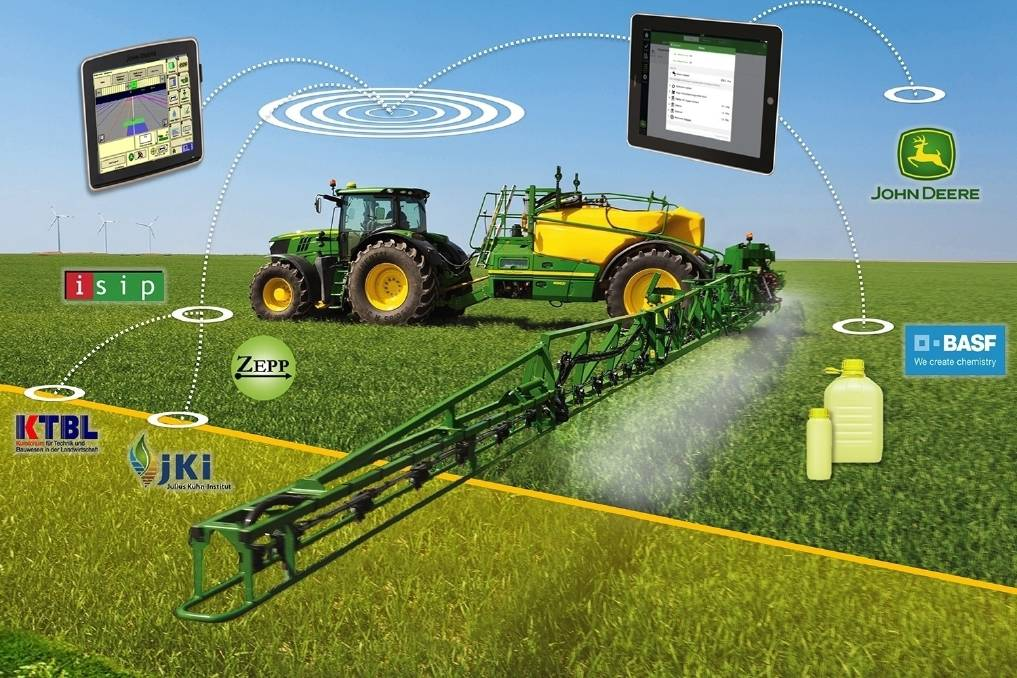
\includegraphics[height=1.0\textheight]{../img/farming}
% \end{frame}
% }


\newcommand{\Section}[1]{\titleimagecolor{red}\section{#1}}

\newcommand{\code}{\lstinline[basicstyle=\ttfamily]}

\newenvironment{Slide}[1]%
  {\begin{frame}[environment=Slide]{#1}}
  {\end{frame}}%



% \newenvironment{Slide}[2][]  /// AAARGH strange error???
%   {\begin{frame}[fragile,environment=Slide,#1]{#2}}
%   {\end{frame}}



\begin{document}

\TitleSlide

%%%%%%%%%%%%%%%

\begin{Slide}{Agenda: workshop om digitalisering}
\begin{itemize}
    \item 13.15 - 13.35  \textbf{Inledning}: Digitalisering - vad och varför?  \\ Prof. Björn Regnell, vicerektor för digitalisering vid LTH

    \item 13.35-14.15 \textbf{Domänspecifika exempel} inom Kemi och Biotekni:
    \begin{itemize}
      \item 13.35 - 13.55   Competence and resources needed for Bioinformatics  \\ Ashfaq Ali, Bioinformatician, NBIS/Immunuotechnology, LTH
      \item 14.00 - 14.15  Avancerad kromatografisk rening - mjukvaror \& digitalisering \\ Dr Niklas Andersson, Kemiteknik, LTH
    \end{itemize}
    
    \item 14.15 - 14.45  \textbf{Gruppdiskussioner}: 
    Hur påverkar digitaliseringen
    \begin{itemize}
      \item Era produkter/tjänser/verksamheter i närtid / på sikt?
      \item Ert behov av kompetens i närtid / på sikt?  
    \end{itemize}



    \item  14.45 - 15.00 \textbf{Sammanfattning}: Hur påverkar detta våra program?
\end{itemize}

~\\Dessa bilder finns här:  
\url{https://github.com/bjornregnell/ws-dig}
\end{Slide}

\section{Inledning}

\begin{Slide}{Vad är digitalisering?}
  \begin{itemize}\small
      \item Digitalisering är processen att införa ny informationsteknologi (IT) i
      verksamheter. 
      \item Digitalisering av samhällen, organisationer och
      branscher avser \textbf{genomgripande verksamhetsomvandling} i samband
      med \textbf{ökad användning av modern IT} \\ och fortsatt övergång till
      \textbf{informationssamhället}. 
      
      \item Denna verksamhets- eller processdigitalisering innefattar ändrade arbetsmetoder,
      organisationsprocesser, affärsmodeller, samhällsstrukturer och
      \textbf{kompetenskrav}.
    \end{itemize}

    \begin{itemize}\small
      \item[]  ~\\\url{https://sv.wikipedia.org/wiki/Digitalisering}
      \item[]  \url{https://en.wikipedia.org/wiki/Digitization}
  \end{itemize}
\end{Slide}


\begin{Slide}{Vad är digitalisering?}
  \begin{itemize}
    \item[(1)] Symbolisk representation, t.ex. färger, ljud, bilder, text
    \item[(2)] Samhällsomvandling genom datateknik
  \end{itemize}
  \pause
  \vspace{1em}
  Teknikutveckling genom historien:
  \begin{itemize}
    \item Domesticering  \hfill 10000 år sedan
    \item Mekanisering \hfill 500 år sedan
    \item Elektrifiering \hfill 250 år sedan
    \item Datorisering \hfill 50 år sedan
    \item Digitalisering  \pause\hfill 25 år sedan... \hfill
    \begin{itemize}
      \item[] -- hela samhällets omvandlas från analogt till digitalt
      \item[] -- sammanvävda IT-system i nästan alla verksamheter
      \item[] -- sensorer och mjukvara nästan överallt
      \item[] -- kompetensgränsöverskridande maktförskjutning
    \end{itemize}
  \end{itemize}
  \end{Slide}
  


\begin{Slide}{Digitaliseringens framgångsfaktorer}
  För framgångsrik och samhällsnyttig digitalisering krävs...
  \begin{itemize}
    \item  en \textbf{kombination} av
    \begin{itemize}
      \item djup domänkunskap
      \item djup kunskap om informationsteknik
    \end{itemize}
    \item förmåga till gränsöverskridande samverkan
    \item förmåga att i ljuset av teknikens möjligheter i grunden omvärdera arbetssätt, värdekedjor, processer, affärsmodeller,, ... (det som brukar kallas \emph{disruptiv innovation})
    \item förmåga att prova sig fram steg för steg och lära av sina misstag (det som brukar kallas \emph{iterativ} eller \emph{agil} systemutveckling
    \item förmåga att göra bra avvägningar mellan olika kavalitetsaspekter (säkerhet, användbarhet, transparens, integritet, tillförlitlighet, prestanda, ...)
  \end{itemize}
  
\end{Slide}


\begin{Slide}{Exempel på utmaningar för alla verksamheter i alla samhällsektorer}
  \begin{itemize}
    \item Hur hantera \textbf{kompetensbristen} inom IT?
    \item Hur hantera den ständigt ökande \textbf{mjukvarukomplexiteten}?
    \item Hur hänga med i den \textbf{allt snabbare} digitala transformationen? \\ Disruptiva affärsmodeller, stordriftsfördelar, innovationsförmåga, ... 
    \item Hur förhålla sig till de stora \textbf{plattformsföretagens} ständigt ökande makt? \\ 
          Usa: Google, Amazon, Facebook, Apple, Microsoft \hfill(GAFAM)\\
          Kina: Baidu, Alibaba, Tencent, JD.com, Didi \hfill (BAT) \\
          Exempel: Facebook vill starta eget virtuellt valutaområde \hfill (Libra)
    \item Hur förhålla sig till alla etiska, juridiska och politiska ödesfrågor?
  \end{itemize}
\end{Slide}

\begin{Slide}{Teknik som möter (några av) utmaningarna}
  \begin{itemize}
    \item \textbf{Öppen källkod} för gemensam infrastruktur och kompetensdelning (github)
    \item \textbf{Abstraktion} av dedicerade funktioner (mikrotjänster, virtualisering)
    \item \textbf{Distribuerad databehandling} med massiv parallellism (''molnet'', beräkningskluster)
    \item (Mjuvaru-ro)\textbf{botar} som tränas med stordata för \textbf{automatiska beslut} (AI, ML)
  \end{itemize}
  ~\\Har din verksamhet egen djup teknisk kompetens inom dessa områden?
\end{Slide}

\ImgFillH{ibm3090}
\ImgFillH{lulea-datacenter}
\ImgFillH{micro-service}
\ImgFillH{farming}
\ImgFillH{helix-nano}
\ImgFillH{ibm-red-hat}
\ImgFillV{ms-github}



\begin{Slide}{Återkommande larm om kompetensbrist (2018)}

\includegraphics[height=0.75\textheight]{../img/kompetenslarm-cio}
\end{Slide}

\begin{Slide}{Återkommande larm om kompetensbrist (2017)}

\includegraphics[height=0.75\textheight]{../img/kompetenslarm-cs}
\end{Slide}

\begin{Slide}{Universiteten levererar inte (än)}
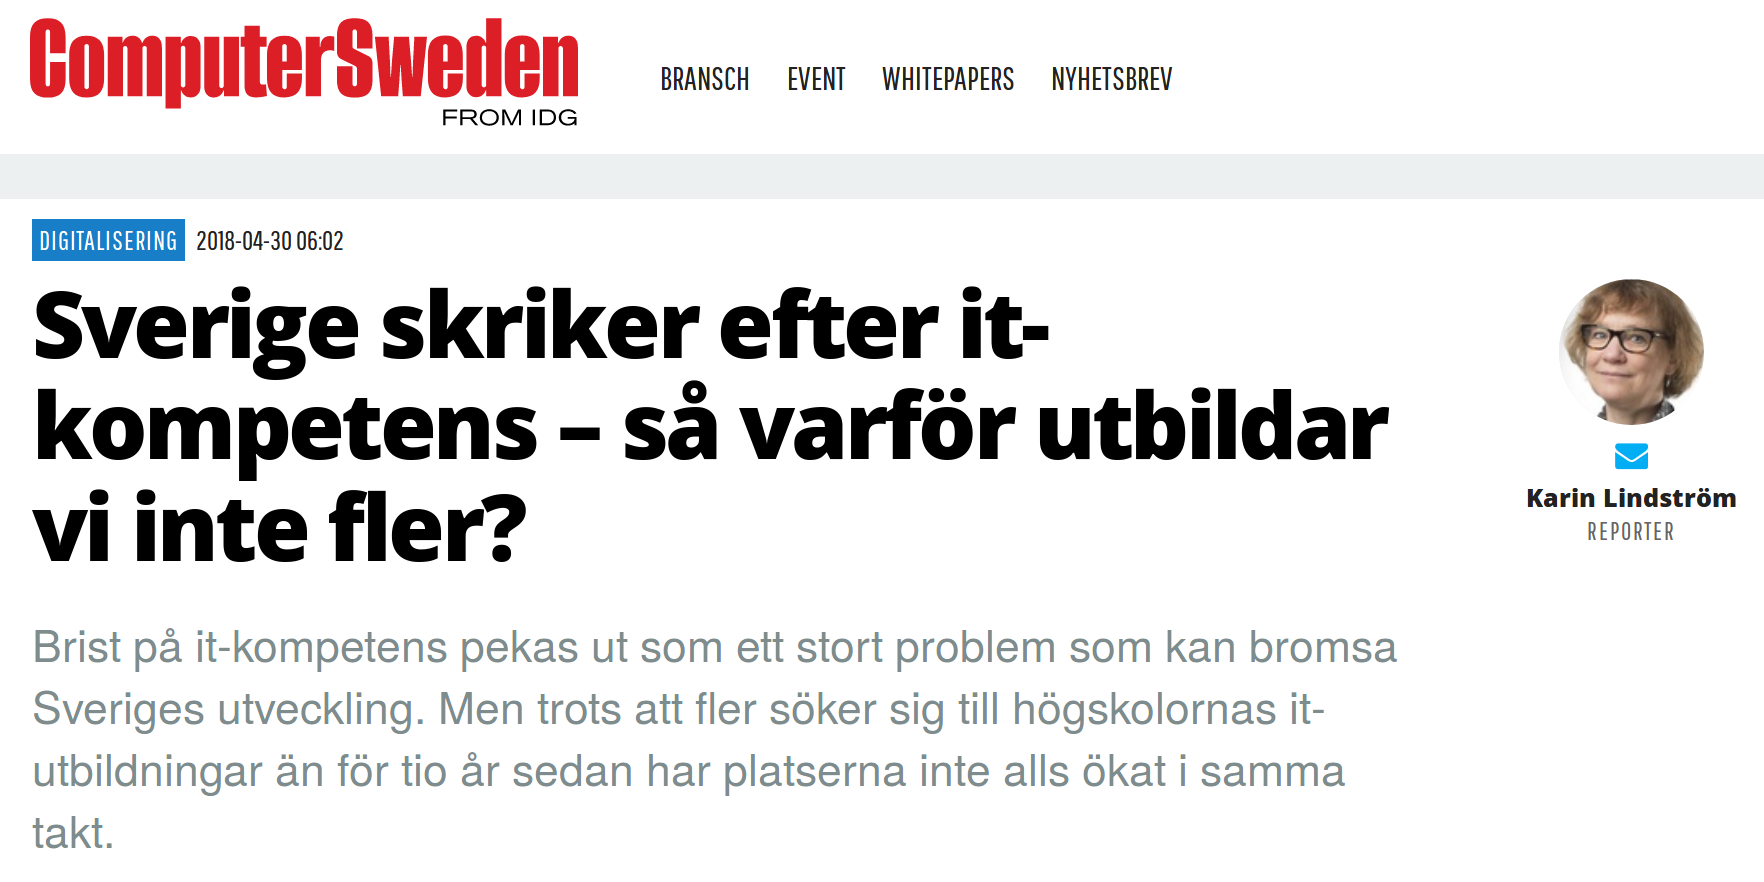
\includegraphics[height=0.75\textheight]{../img/utbilda-fler}
\end{Slide}


\begin{Slide}{LTH:s framtida konkurrenter?}
  \begin{minipage}{0.23\textwidth}
  \begin{itemize}
    \item Amazon
    \item Facebook
    \item Google
  \end{itemize}
  \end{minipage}
  \begin{minipage}{0.7\textwidth}
    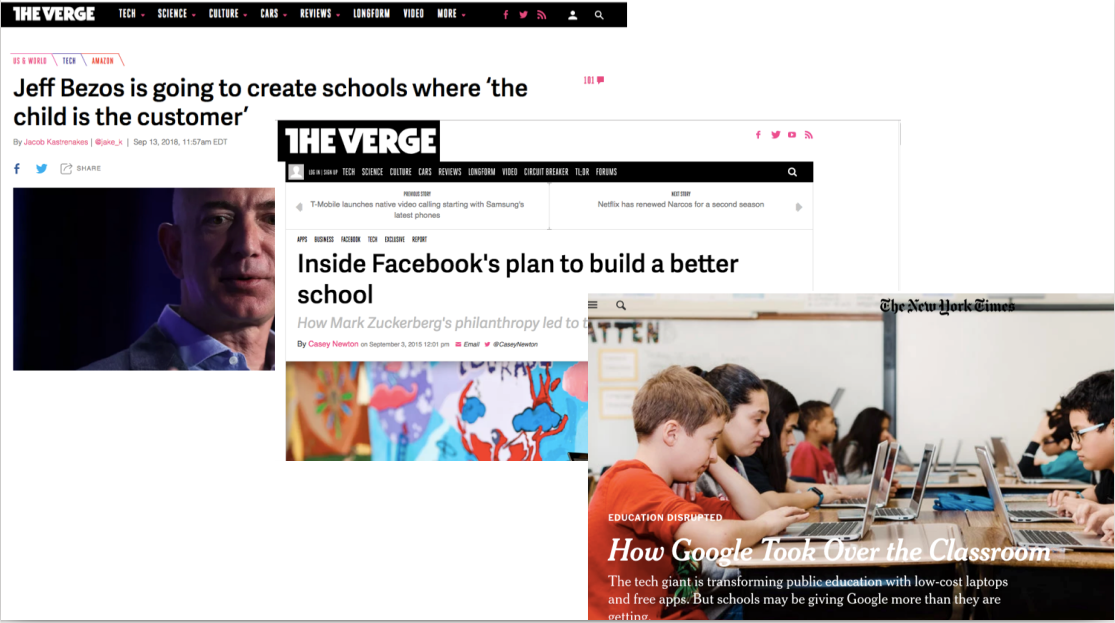
\includegraphics[height=0.85\textheight]{../img/afg}
  \end{minipage}
\end{Slide}

\begin{frame}[plain]

\includegraphics[height=1.3\textheight]{../img/aws}
\end{frame}


\begin{Slide}{Exempel på input från näringslivet}
  Några axplock ur förslagen i rapport från Swedsoft: \\''Kan Sverige vara världsledande på mjukvaruutveckling och -forskning i framtiden?''\\
  \href{https://www.swedsoft.se/wp-content/uploads/sites/7/2019/09/Swedsoft-Helhetssyn-p\%C3\%A5-mjukvarans-betydelse-f\%C3\%B6r-digitalisering-och-konkurrenskraft.pdf}{www.swedsoft.se, 2019-09-04}
\begin{itemize}
  \item Det krävs ekonomiska förutsättningar för lärosätena att arbeta med yrkesverksamma.
  \item Nationellt kunskapslyft för att stimulera kompetenshöjningar, även på grundläggande högskolenivå och för personer med olika utbildningsbakgrund.
  \item Stipendier till utvalda mjukvaruutbildningar för utländska studenter, som garanteras att få stanna kvar i Sverige under en längre period efter utbildningen.
  \item Brett forskningsprogram inom mjukvaruutveckling där forskning sker i samverkan med företag, öppet för alla lärosäten med minst ett treårigt mjukvaruutvecklings- eller datavetenskapligt utbildningsprogram.
\end{itemize}
\end{Slide}

\begin{Slide}{Exempel på grundkunskaper inom IT}
\begin{itemize}
  \item Programmering
  \item Systemutvecklingsmetodik
  \item Datastrukturer, databaser
  \item IT-säkerhet (security/datasäkerhet, safety/personsäkerhet, ...)
  \item Kommunikationsnätverk
  \item Distribuerade beräkningar
  \item ...
\end{itemize}  
Digitaliseringskunskapsbehov i undervisningen:\\Vad behöver ingå i utbildningsprogram X?
\end{Slide}



\section{Diskussion}

\begin{Slide}{Diskussion}
  \begin{itemize}
    \item Näringslivrepresentanter: Hur påverkar digitaliseringen...
    \begin{enumerate}
        \item  ...era \textbf{produkter/tjänster/verksamheter} i
        närtid / på sikt?
        
        \item ...ert \textbf{behov av kompetens} i närtid / på
        sikt?
    \end{enumerate}
    \item Studentrepresentanter: vilken kompetens ni tror ni kommer att behöva, och vad som vore bra att få in i er utbildning?
  \end{itemize}
\end{Slide}

\EndSlide

\end{document}